\documentclass{beamer}
%
% Choose how your presentation looks.
%
% For more themes, color themes and font themes, see:
% http://deic.uab.es/~iblanes/beamer_gallery/index_by_theme.html
%
\mode<presentation>
{
  \usetheme{Warsaw}      % or try Darmstadt, Madrid, Warsaw, ...
  \usecolortheme{default} % or try albatross, beaver, crane, ...
  \usefonttheme{default}  % or try serif, structurebold, ...
  \setbeamertemplate{navigation symbols}{}
  \setbeamertemplate{caption}[numbered]
} 

\usepackage{minted}
\usepackage[english]{babel}
\usepackage[utf8x]{inputenc}
\usepackage[absolute,overlay]{textpos}

\title[Blender Intro]{Introduction to Blender}
\author{Łukasz Hryniuk}
\date{\today}

\begin{document}

\begin{frame}
  \titlepage
  \centering\href{https://github.com/hryniuk/blender-intro}{github.com/hryniuk/blender-intro}
\end{frame}

\begin{frame}{Outline}
  \tableofcontents
  
  \centering \Large It won't cover texturing and animation
\end{frame}

\section{Introduction}

\begin{frame}{About me and you}

\begin{itemize}
\item About me
\item About you
\item Number of Blender copies?
\end{itemize}

\end{frame}

\begin{frame}{Goal}

\centering \Huge
\emph{Blender is not so hard to learn and worth trying}

\end{frame}

\begin{frame}{What's Blender}

\begin{itemize}
  \item \textbf{allows Python scripting} (next time)
  \item beside 3D modelling also video editing (nice example: rotoscoping), game engine and \href{https://www.youtube.com/watch?v=L1Wl3YoRe8w}{2d animation} (to be improved in Blender 2.8)
  \item free software
  \item alternative to e.g. 3DS Max and Maya
\end{itemize}

\begin{figure}

\includegraphics[scale=0.15]{logo.png}
%\caption{\href{https://www.blender.org/}{Blender's logo}}
\end{figure}

\end{frame}

\begin{frame}{Motivation}

Two examples - how Blender may help you and what's possible:
\begin{itemize}
\item \href{https://www.cv.nrao.edu/~bkent/blender/index.html}{3D Scientific Visualization with Blender} - book and tutorials
\item \href{https://agent327.com/}{Agent 327: Operation Barbershop} - “the Netherlands’ answer to James Bond"
\end{itemize}

\end{frame}

\section{Interface and modes}

\begin{frame}{Blender interface}

\begin{figure}
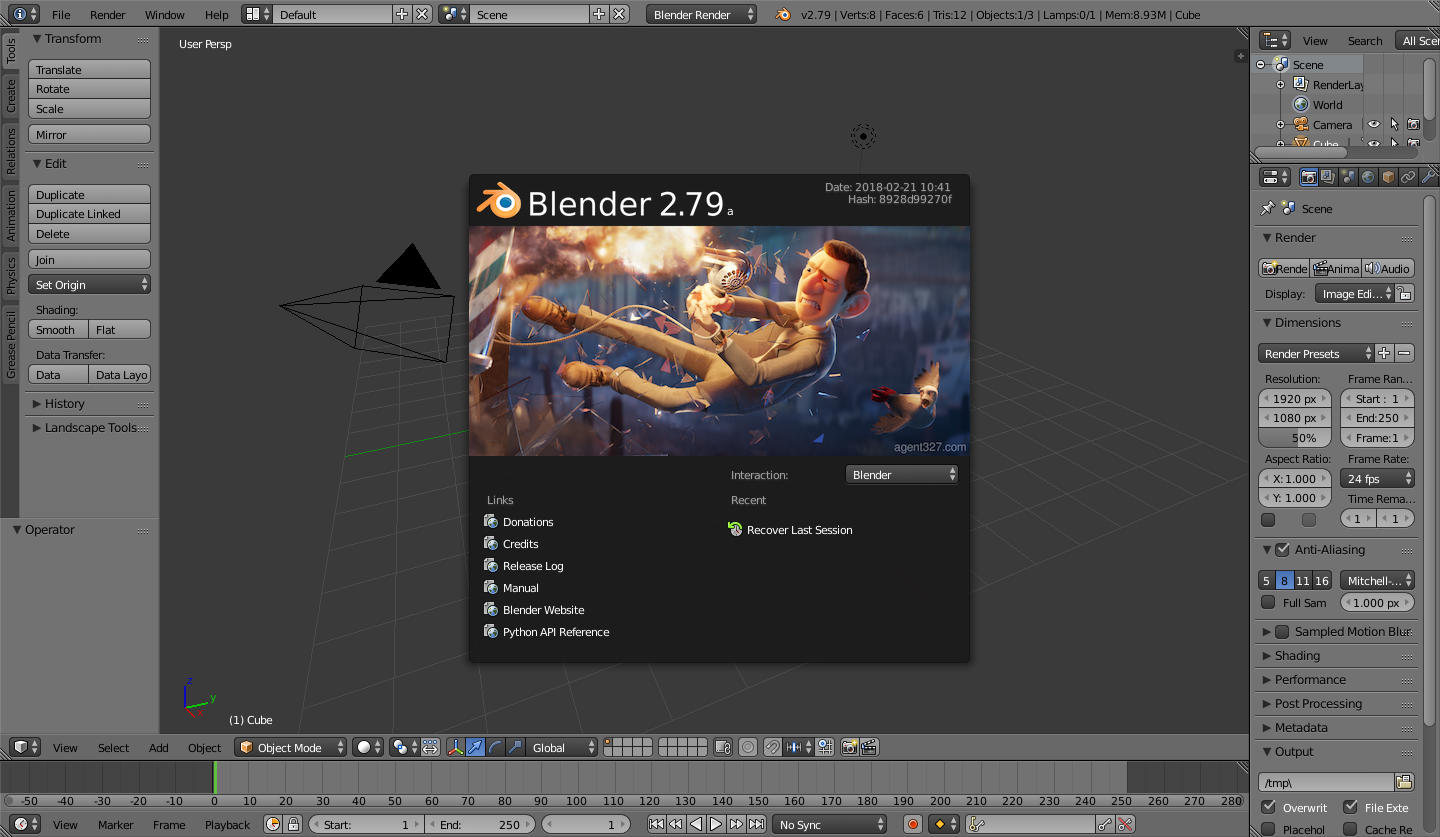
\includegraphics[scale=0.25]{interface.png}
%\caption{Version 2.79, Wikipedia}
\end{figure}

...may be a bit intimidating. We'll go through it in the minute.

\end{frame}

\begin{frame}{Three essential modes}

% TODO: add descriptions to these modes
\begin{itemize}
\item Object - object datablock edition
\item Edit - parts of the mesh (curves and surfaces) edition
\item Sculpt - mesh sculpting (more or less "area-based" mesh edition)
\end{itemize}

\end{frame}

\begin{frame}{First demo}

\centering \Huge
\emph{Let's get familiar with it}

\end{frame}

\section{Shortcuts and editing}

\begin{frame}{How we can edit objects?}
In fact 12 shortcuts + mouse are enough
to do most of the things efficiently. Starting from \textbf{object mode}:
\begin{itemize}
\item \textbf{G}rab
\item \textbf{S}cale
\item \textbf{R}otate
\item \textbf{Shift+A}(dd)
\item \textbf{X} (Cut, of course)
\item Select \textbf{A}ll
\end{itemize}

\end{frame}


\begin{frame}{How we can edit objects?}

...and in edit mode (switch it with \textbf{TAB}):
\begin{itemize}
\item Add \textbf{F}ace
\item \textbf{E}xtrude
\item \textbf{B} - rectangle selection tool
\item \textbf{C}yclic selection tool
\item \textbf{K}nife
\item \textbf{W} - edit mode popup menu (with operations like Subdivide, Smooth, Bevel and Symmetrize)

\end{itemize}

\end{frame}

\begin{frame}{How we can edit objects?}

\centering \Large
{Beside that, one can also use modifiers available in a separate tab (under shortcuts too): Array, Boolean, Screw and Soldify to name a few}

\end{frame}

\begin{frame}{Second demo}

\centering \Huge
\emph{Back to Blender}

\end{frame}

\section{Rendering}

\begin{frame}{Rendering engines - how to get an image from the scene?}

Just press \textbf{F12}. There are three rendering engines in Blender (you can get more with Add-ons):
\begin{itemize}
\item Blender Render - the oldest and the simplest
\item Blender Game - for the Blender Game Engine; designed for interactive use
\item \textbf{Cycles Render} - physically based production renderer for photorealistic images
\end{itemize}

\end{frame}

\begin{frame}{Blender Render vs Cycles Render}

\begin{textblock*}{6cm}(0.2cm,2cm) % {block width} (coords)
\begin{figure}
\includegraphics[scale=0.6]{blender_render.png}
\end{figure}
\end{textblock*}

\begin{textblock*}{6cm}(6.5cm,2cm) % {block width} (coords)
\begin{figure}
\includegraphics[scale=0.6]{cycles_render.png}
\end{figure}
\end{textblock*}

\end{frame}

\begin{frame}{Third demo}

\centering \Huge
\emph{Let's play with Cycles}

\end{frame}


\begin{frame}{Learning resources}

\begin{itemize}
\item \href{https://www.blenderguru.com/}{Blender Guru tutorials}
\item \href{https://www.blender.org/support/tutorials/}{Blender.org tutorials}
\item \href{http://polskikursblendera.pl/}{Polski Kurs Blendera}
\end{itemize}

\end{frame}

\begin{frame}{}
  \centering \Huge
  \emph{Questions, comments and feedback}
\end{frame}

\begin{frame}{}
  \centering \Huge
  \emph{Thank You}
\end{frame}

\end{document}
